
Les données et les questions de cet exercice concernent la France métropolitaine.

\begin{center}
\begin{tabularx}{\linewidth}{|m{8cm}|X|}\hline

\multicolumn{1}{|c|}{Document 1}&\multicolumn{1}{|c|}{Document 2}\\

En 2015, environ 4,7\,\% de la population française souffrait d'allergies alimentaires.

En 2010, les personnes concernées par des allergies alimentaires étaient deux fois moins nombreuses qu'en 2015.

En 1970, seulement 1\,\% de la
population était concernée.

{\footnotesize \emph{Source : Agence nationale de la sécurité sanitaire de l'alimentation, de l'environnement et du
travail.}}&

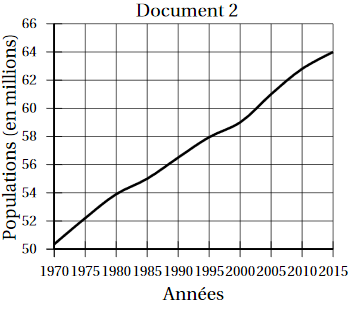
\includegraphics[scale=0.8]{NF-44.png} 


\end{tabularx}
\end{center}

\begin{enumerate}
\item Déterminer une estimation du nombre de personnes, à 100 000 près, qui souffraient d’allergies alimentaires en France en 2010.
\item Est-il vrai qu’en 2015, il y avait environ 6 fois plus de personnes concernées qu’en 1970?
\end{enumerate}